\documentclass[11pt,letterpaper]{article}

\usepackage[margin=1in]{geometry}
\usepackage[T1]{fontenc}
\usepackage[utf8]{inputenc}
\usepackage{lmodern}
\usepackage{microtype}
\usepackage{amsmath,amssymb,mathtools,bm}
\usepackage{booktabs,tabularx,array}
\usepackage{xcolor}
\usepackage[most]{tcolorbox}
\usepackage{enumitem}
\usepackage{fancyhdr}
\usepackage{tikz}
\usetikzlibrary{calc, arrows.meta, positioning, fit, backgrounds, shapes.geometric}
\usepackage[hidelinks]{hyperref}

\definecolor{deepblue}{RGB}{25,55,90}
\definecolor{softblue}{RGB}{236,244,250}
\definecolor{softgreen}{RGB}{237,247,239}
\definecolor{softorange}{RGB}{252,244,231}
\definecolor{softgray}{RGB}{244,244,244}
\definecolor{deepgreen}{RGB}{30,90,45}

\hypersetup{
  pdftitle={Pointwise Meta-Agent Renormalization: A Physicist's Guide},
  pdfauthor={MultiAgentELBO project},
  pdfsubject={Gauge transport, coarse graining, variational free energy, and meta-agent construction}
}

\pagestyle{fancy}
\fancyhf{}
\lhead{\textit{Pointwise meta-agent renormalization}}
\rhead{\textit{Physicist's guide}}
\cfoot{\thepage}
\setlength{\headheight}{14pt}

\setlength{\parindent}{0pt}
\setlength{\parskip}{0.7em}
\setlist[itemize]{leftmargin=1.6em,itemsep=0.25em,topsep=0.25em}

\newcommand{\KL}{\operatorname{KL}}
\newcommand{\Prob}{\mathbb P}
\newcommand{\Rec}{\mathbb Q}
\newcommand{\Post}{\boldsymbol\Pi}
\newcommand{\Law}{\mathcal P}
\newcommand{\id}{\operatorname{id}}
\newcommand{\ev}{\operatorname{ev}}

\newtcolorbox{physicalreading}{
  colback=softblue,
  colframe=deepblue,
  title=Physical reading,
  fonttitle=\bfseries,
  breakable
}

\newtcolorbox{provedbox}{
  colback=softgreen,
  colframe=green!45!black,
  title=What is established,
  fonttitle=\bfseries,
  breakable
}

\newtcolorbox{boundarybox}{
  colback=softorange,
  colframe=orange!65!black,
  title=Boundary of the result,
  fonttitle=\bfseries,
  breakable
}

\newtcolorbox{translationbox}{
  colback=softgray,
  colframe=black!55,
  title=Translation,
  fonttitle=\bfseries,
  breakable
}

\title{\textbf{Pointwise Meta-Agent Renormalization}\\[0.35em]
\Large A Physicist's Guide to the Static Theory}
\author{MultiAgentELBO theory program}
\date{August 15, 2026}

\begin{document}

\maketitle

\begin{abstract}
This document explains the pointwise meta-agent renormalization result in the language of effective theories, gauge transport, information loss, and coarse observables. The central construction takes a block of fine agents and one declared coarse channel, then produces a normalized parent generative law, recognition law, and posterior law. An exact relative-entropy chain rule measures the information discarded by that channel. The result is static and pointwise: it holds at one base point, one structural configuration, and one admitted observation. It does not yet construct a spacetime-dependent geometric agent, autonomous dynamics, nonequilibrium persistence, or a unique microscopic physics.
\end{abstract}

\tableofcontents
\newpage

\section{The theory in one page}

The renormalization question is familiar from physics: if a set of microscopic degrees of freedom is replaced by an effective degree of freedom, what information survives, what information is lost, and which predictions remain unchanged? Here the microscopic objects are agents carrying probabilistic beliefs and generative-model presentations. The effective object is called a candidate parent or meta-agent datum.

There are two complications beyond ordinary block-spin language. First, different agents may express their states in different local frames. Their probability laws cannot be compared until they are transported into a common frame. Transport around a closed loop can return a state in a rotated or otherwise transformed frame; this is the holonomy. Second, the object being coarse-grained is not a single field value. It is a probabilistic triple:
\[
  \text{generative law } \Prob_I,
  \qquad
  \text{recognition law } \Rec_{I,o,X},
  \qquad
  \text{posterior } \Post_{I,o,X}.
\]
The subscript \(I\) denotes the fine block, \(X\) is fixed structural data, and \(o\) is the admitted observation. Section~\ref{sec:four-objects} defines each of these three laws, together with the Markov channel introduced next; a reader meeting the vocabulary for the first time should start there.

One normalized Markov channel \(C_A\) is applied to the fine latent variables. The same channel must be used for recognition and posterior. It is chosen independently of the current recognition law, posterior, parameters, and observation. The parent triple is
\begin{equation}
  \Rec_{A,o,X}=\Rec_{I,o,X}C_A,
  \qquad
  \Prob_A=(\id_{\mathsf O}\times C_A)_{\#}\Prob_I,
  \qquad
  \Post_{A,o,X}=\Post_{I,o,X}C_A.
  \label{eq:parent-triple}
\end{equation}
The observation coordinate is not coarse-grained, and the structural variable \(X\) remains an external conditioning datum. Equation~\eqref{eq:parent-triple} is the probabilistic core of the static meta-agent construction.

The exact information balance is
\begin{equation}
  \KL(\Rec_{I,o,X}\Vert\Post_{I,o,X})
  =
  \KL(\Rec_{A,o,X}\Vert\Post_{A,o,X})
  +\Delta_A(o,X),
  \qquad
  \Delta_A(o,X)\geq 0.
  \label{eq:kl-chain-preview}
\end{equation}
The nonnegative term \(\Delta_A\) is the recognition-versus-posterior information that remains in the fine variables after the parent variable is known. It is the exact cost of forgetting those variables for this pair of laws.

\begin{physicalreading}
The theorem is an exact static coarse-graining statement. It resembles an RG step because a block is mapped to an effective probabilistic description and the discarded information is quantified. It is not yet a dynamical RG flow, a continuum limit, or a derivation of agency.
\end{physicalreading}

\section{The four objects}
\label{sec:four-objects}

Everything in this document is built from four things. Three of them are probability laws that describe one scale, and the fourth is the map that carries one scale to the next. Because the rest of the argument is bookkeeping about how those four interact, it is worth stating each one carefully before any theorem is quoted.

\textit{The generative law} \(\Prob_I(do,dy\mid X)\) is the model of the world. It is a single normalized probability measure on the product of the observation space \(\mathsf O\) and the fine latent space \(\mathsf Y_I\), conditioned on the structural data \(X\) and on the numerical parameters. It plays the role that an action or a Gibbs measure plays in statistical physics: it is the declared account of how configurations arise, written down once, before any inference is attempted. Its arguments are the parameters and \(X\), and nothing else. That typing restriction is load bearing rather than stylistic. If a factor of the generative law were permitted to read the current recognition law, the joint would move whenever the inference moved, and there would be no fixed evidence against which an improvement could be certified. This is why the generative law is fixed before recognition is chosen.

\textit{The recognition law} \(\Rec_{I,o,X}(dy)\) is the belief the block currently holds about the latent state, given that the observation \(o\) has been admitted and the structural data \(X\) is in force. It is a normalized measure on the latent space alone, and it is indexed by \((o,X)\) because it must return a different answer for each observation and each structural configuration. It is an approximation, and it is not required to agree with anything. It is also permitted to correlate the child agents with one another and the belief channel with the model channel. The theory carries it as one correlated joint object rather than as a list of per-agent marginals, because those correlations are exactly what a list of marginals would destroy.

\textit{The posterior} \(\Post_{I,o,X}(dy)\) is what the generative law itself implies about the latent state once \(o\) has been seen. It is the conditional of \(\Prob_I\) on the observation coordinate, and it is the Bayesian target that recognition is trying to match. The qualifier ``selected version'' in the technical statements is not decoration. A conditional probability is determined by a joint law only up to a set of observations of probability zero, so at an exceptional observation the joint law fixes no pointwise conditional at all. The theory therefore declares one measurable representative and uses that representative consistently; every statement about \(\KL(\Rec\Vert\Post)\) below is a statement about the declared version, and is an almost-sure statement in the observation.

\textit{A Markov channel} is not a law but a map between scales. A normalized Markov channel \(C_A(dz\mid y)\) from the fine latent space to the parent latent space is a rule that is measurable in \(y\) and, for each fixed \(y\), is a normalized probability measure in \(z\). It carries a law forward by
\[
  (\Rec C_A)(dz)=\int_{\mathsf Y_I}\Rec(dy)C_A(dz\mid y).
\]
The word ``normalized'' is what separates a channel from a bare aggregation matrix, an energy restriction, or a Galerkin projection: total probability is preserved rather than created or destroyed. The channel is the block-spin rule of this theory. It may be deterministic, in which case it is a hard assignment of fine states to parent states, or genuinely stochastic, in which case it behaves like a noisy detector; and it is allowed to discard almost everything.

The single structural rule tying the four together is that exactly one channel is used. The same \(C_A\) acts on the generative law, the posterior, and the recognition law, and it is chosen without reference to the current recognition law, posterior, parameters, or observation. A channel allowed to depend on the recognition law would be a parameter-dependent model transformation rather than one channel between two experiments, and the information identity of Section~\ref{sec:info-cost} would not follow.

\begin{translationbox}
The generative law is the declared action or Gibbs measure. The recognition law is the trial or variational ansatz. The posterior is the exact conditional that the ansatz is trying to reproduce. The Markov channel is the blocking rule. The theorem then says what happens to all four when the blocking rule is applied.
\end{translationbox}

\section{A physics dictionary}

\begin{table}[ht]
\centering
\small
\begin{tabularx}{\textwidth}{>{\raggedright\arraybackslash}p{0.19\textwidth}X}
\toprule
\textbf{Symbol or term} & \textbf{Physical interpretation} \\
\midrule
\(\mathcal C\) & Contextual base space. A point of \(\mathcal C\) specifies where the local probabilistic data are evaluated. It need not be physical spacetime. \\
\(\mathcal C_i\) & Region on the base over which agent \(i\) is defined. \\
\(\mathcal U_A=\bigcap_{i\in I}\mathcal C_i\) & Common overlap patch for a finite child block \(I\) and candidate parent label \(A\). \\
\(r_*\) & One fixed point in the overlap. The proved construction is performed in the fiber over this point. \\
Law & A normalized probability measure on a declared measurable state space. It is a generic type, not one special global object. \\
\(\Prob\) & The generative law: the model's normalized joint distribution over observations and latent variables, conditional on declared structural data. \\
\(\Rec\) & The recognition law: the agent's current inferential distribution over latent variables for an admitted observation. \\
\(\Post\) & A selected posterior version obtained from the generative law. It is the Bayesian target against which \(\Rec\) is compared. \\
\(m\in\mathsf M_i\) & A model presentation or model-valued state. It becomes an operative generative mechanism through an evaluation map \(m\mapsto K_m\). \\
\(q_i^m\) & A probability law over model presentations. A sharp model is the special case \(q_i^m=\delta_m\). \\
\(\Omega_{ij}\) & Transport from agent \(j\)'s local frame to agent \(i\)'s local frame. \\
\(H\) & Holonomy: the ordered product of transports around a closed path. \\
\(H_{\#}Q=Q\) & The law \(Q\) is invariant under the loop transformation. This is weaker than \(H=I\). \\
\(\eta_{ij}=\alpha_i\beta_{ij}\) & Joint probability of the directed edge event ``receiver \(i\), source \(j\).'' \\
\(C_A\) & The normalized coarse Markov channel that turns the fine latent state into the parent latent state. \\
\(\Delta_A\) & Conditional relative entropy discarded by the coarse channel. \\
\(\mathcal F\) & Variational free energy at fixed evidence, equal to a KL term plus the common evidence contribution. \\
\bottomrule
\end{tabularx}
\caption{A translation between the repository notation and standard physics language.}
\label{tab:dictionary}
\end{table}

\subsection{What ``law'' means}

A law is simply a normalized probability measure. The phrase can refer to the global generative law \(\Prob\), the global recognition law \(\Rec\), a posterior \(\Post\), an agent's local belief law, or a distribution over model presentations. The symbols \(\Prob\) and \(\Rec\) name particular roles; they do not exhaust the meaning of ``law.''

For example, \(q_i^m\in\Law(\mathsf M_i)\) is a law over the model fiber \(\mathsf M_i\). A point \(m\in\mathsf M_i\) is one model presentation. Turning that presentation into an operative mechanism is the job of the evaluation map, which the next subsection describes.

\subsection{Kernels, presentations, and the evaluation map}
\label{sec:ev}

A \emph{kernel} is a conditional law carrying a measurability requirement. A kernel \(K\) from a source space \(\mathsf S\) to a target space \(\mathsf T\) assigns to each source point \(u\in\mathsf S\) a probability measure \(K(u,dt)\) on \(\mathsf T\), in such a way that \(u\mapsto K(u,B)\) is measurable for each fixed measurable set \(B\). Informally, a kernel is a probability distribution that depends measurably on an input, and a law is the degenerate case of a kernel with no input. The Markov channel \(C_A(dz\mid y)\) of Section~\ref{sec:four-objects} is a kernel; so is a transition mechanism, an observation mechanism, and a posterior version regarded as a function of the observation.

A \emph{generative kernel} is one of the conditional factors out of which the generative law is assembled. The declared factorization orders the agents along a directed acyclic graph and writes the joint law as an ordered composition of normalized kernels, one per agent and design point. The kernel \(K_{i,m}^{X}\) is agent \(i\)'s factor: it takes the source coordinates that the declared factorization says agent \(i\) depends on, namely its parent latents and any observation coordinates it reads, together with the structural data \(X\), and returns a normalized law over agent \(i\)'s own output coordinates. Composing these factors is what produces \(\Prob\), and the composition normalizes exactly, with no partition function to compute.

The map
\[
  \ev_i:m\longmapsto K_{i,m}^{X}
\]
is the \emph{evaluation map}, and it converts a model presentation into the mechanism that presentation denotes. The useful analogy is that \(m\) is source code or a parameter vector, \(K_{i,m}^{X}\) is the running program, and \(\ev_i\) is the act of compiling and instantiating it. Three types are involved and they are easy to conflate. The object \(q_i^m\) is a law over presentations; the object \(m\) is a single presentation, which is a sample and never a law; and \(K_{i,m}^{X}\) is a kernel, which is a function rather than a point. Neither the law over presentations, nor a recognition parameter, nor a posterior is ever an argument of the evaluated generative kernel; the typing prohibition of Section~\ref{sec:four-objects} applies here too.

The reason for keeping the presentation separate from the kernel it evaluates to is that the theory wants agents to hold beliefs \emph{about models}, and a belief about a model needs a measurable space of models on which to place a law. The space of kernels is an awkward object to do this on, whereas a space of presentations can simply be declared standard Borel. The map \(\ev_i\) then supplies the bridge. It need not be injective: two distinct presentations can compile to the same kernel. One is free to declare \(m\sim m'\) when their evaluated kernels agree, but the measurability of \(\ev_i\) does not by itself supply standard-Borel, Hausdorff, or smooth regularity of the resulting quotient, and no such regularity is claimed. A quotient-level model fiber would need a separate theorem, so the default construction retains presentations rather than working with equivalence classes. The same construction is used one scale up, where \(\ev_A\) is the parent evaluator discussed in Section~\ref{sec:parent-evaluator}.

The general theory therefore uses measurable model spaces, and smooth statistical manifolds when differential structure is needed. Multivariate Gaussians are optional finite computational realizations, not the definition of a model fiber or of an agent.

\section{Gauge transport and network frustration}

\subsection{Why transport is needed}
\label{sec:transport}

Suppose two agents assign probability laws to locally represented states. Directly comparing the coordinate arrays is meaningless if the agents use different frames. A transport map \(\Omega_{ij}:j\to i\) first expresses agent \(j\)'s law in agent \(i\)'s frame. The edge mismatch is then
\[
  \KL\left(p_i\Vert(\Omega_{ij})_{\#}p_j\right).
\]
This is the probabilistic analogue of comparing vectors only after parallel transport.

The theory keeps belief and model transport separate:
\[
  (\beta_{ij},\Omega_{ij})
  \quad\text{and}\quad
  (\gamma_{ij},\widetilde\Omega_{ij}).
\]
The matrices \(\beta\) and \(\gamma\) provide conditional edge weights in the belief and model channels. They describe an informational network, but they do not by themselves establish a unique causal DAG or a unique microscopic physics.

Because every statement below holds verbatim for both channels, it is convenient to carry one channel-generic notation. For \(x\in\{q,m\}\), write \(p_i^x\) for agent \(i\)'s own law in channel \(x\), expressed in agent \(i\)'s own frame and evaluated at the fixed base point \(r_*\); thus \(p_i^q\) is the belief law \(q_i(r_*)\) and \(p_i^m\) is the law over model presentations \(q_i^{m}(r_*)\). Write \(T_{ij}^x\) for the corresponding transport from \(j\)'s frame to \(i\)'s frame, so that
\[
  T_{ij}^q=\Omega_{ij},
  \qquad
  T_{ij}^m=\widetilde\Omega_{ij}.
\]
On every positive-support edge these transports are declared to be bimeasurable bijections satisfying \(T_{ji}^x=(T_{ij}^x)^{-1}\). Reciprocity is what makes composition along a path well defined and makes the reverse path undo the forward path, which is what the holonomy discussion below requires. The bare symbol \(p_i\) used a moment ago is \(p_i^x\) before the channel is named.

\subsection{The joint edge-event law}

A conditional attention row is not yet a normalized law over all directed edges. Let \(\alpha_i^x\) be the normalized probability of sampling receiver \(i\) in channel \(x\). Then
\begin{equation}
  \eta_{ij}^q=\alpha_i^q\beta_{ij},
  \qquad
  \eta_{ij}^m=\alpha_i^m\gamma_{ij}.
  \label{eq:eta}
\end{equation}
Thus \(\eta_{ij}^x\) is the joint probability of observing the directed event ``receiver \(i\), source \(j\).'' In a transformer implementation the receiver occupancy can be fixed externally, often uniformly, and need not be another learned attention parameter. The row \(\beta_{ij}\) or \(\gamma_{ij}\) says which source is selected conditional on the receiver; \(\alpha_i\) says how receivers enter the ensemble.

\subsection{Holonomy is not the same as disagreement}
\label{sec:holonomy}

Transport around a closed path gives a holonomy transformation \(H\). Two logically different statements often get conflated:
\[
  H=I,
  \qquad\text{and}\qquad
  H_{\#}Q=Q.
\]
The first says the frame returns exactly to itself. The second says that the probability law is unchanged by the returned frame transformation. An isotropic distribution can satisfy \(H_{\#}Q=Q\) even for a nonidentity rotation. Conversely, a tree has no nontrivial loops and hence no holonomy obstruction, yet two nodes on the tree can carry completely different laws.

\begin{translationbox}
Holonomy measures path dependence of frame transport. It does not, by itself, measure agreement of the transported states. For a parent that forgets which path was used, \(H_{\#}Q=Q\) is the relevant invariance condition. A richer parent may instead retain the holonomy or path mark as internal state.
\end{translationbox}

\subsection{Zero transported distortion}
\label{sec:zero-distortion}

For channel \(x\in\{q,m\}\), define
\begin{equation}
  \mathcal D_x
  =
  \sum_{i,j:\eta_{ij}^x>0}
  \eta_{ij}^x
  \KL\left(
  p_i^x\Vert(T_{ij}^x)_{\#}p_j^x
  \right).
  \label{eq:distortion}
\end{equation}
This is a nonnegative sum, weighted by the joint edge-event law of Equation~\eqref{eq:eta}, of the transported edge mismatches introduced in Section~\ref{sec:transport}.

To state the consequence, fix a root vertex \(r\) and, for each node \(i\), a path \(\gamma_i\) from \(i\) to \(r\). Write \(T_{\gamma_i}^x\) for the ordered composite of the edge transports along that path, and
\[
  P_i^x:=(T_{\gamma_i}^x)_{\#}p_i^x
\]
for agent \(i\)'s own law re-expressed in the root's frame. On a connected graph a rooted spanning tree supplies such a path for every node; the edges left out of the tree generate the based holonomy group at \(r\), whose elements are the loop transformations \(H\) of Section~\ref{sec:holonomy}.

The result this guide calls the \emph{two-channel zero-distortion theorem} is then the following. On a connected positive-support graph, and for each channel \(x\) separately, these three statements are equivalent: first, \(\mathcal D_x=0\); second, \(p_i^x=(T_{ij}^x)_{\#}p_j^x\) on every positive-weight directed edge; and third, there is a unique law \(Q_x\) with
\begin{equation}
  (T_{\gamma_i}^x)_{\#}p_i^x=Q_x
  \quad\text{for every }i,
  \qquad
  H_{\#}Q_x=Q_x
  \quad\text{for every retained holonomy }H.
  \label{eq:root-law}
\end{equation}
In words, zero total distortion is the same thing as edgewise agreement after transport, and the same thing again as the existence of one path-independent root law lying in the holonomy-fixed sector. Since \(\mathcal D_q\) and \(\mathcal D_m\) are separately nonnegative, their sum vanishes exactly when both vanish, so the equivalence can be applied to \(x=q\) with the pair \((\beta,\Omega)\) and to \(x=m\) with the pair \((\gamma,\widetilde\Omega)\). The output is the typed pair \((Q_q,Q_m)\), one consensus law per channel, which is what the name records.

That pair does not determine a joint belief-model law. Correlations are extra information, and Section~\ref{sec:marginals} makes the failure explicit.

The name itself is this guide's shorthand. The statement above, with the edge-weighted distortion \(\mathcal D_x\), is proved in the 2026-08-14 derivation package rather than in the canonical theory chapters, which carry a related result stated with node weights and a restricted candidate family. Section~\ref{sec:provenance} records the exact provenance, and the phrase should not be confused with the unrelated finite-ELBO decomposition that other project documents also call a two-channel result.

\begin{physicalreading}
Equation~\eqref{eq:distortion} acts like a nonnegative frustration energy on a gauge network. Zero energy means edgewise compatibility and path-independent reconstruction of a root law, provided the root law lies in the holonomy-fixed sector. It does not mean that the connection itself is flat.
\end{physicalreading}

\section{From a fine block to a parent effective description}
\label{sec:parent}

Figure~\ref{fig:parent} shows the whole construction on one page. Everything that follows in this section is a careful reading of that diagram.

\begin{figure}[ht]
\centering
\resizebox{\textwidth}{!}{%
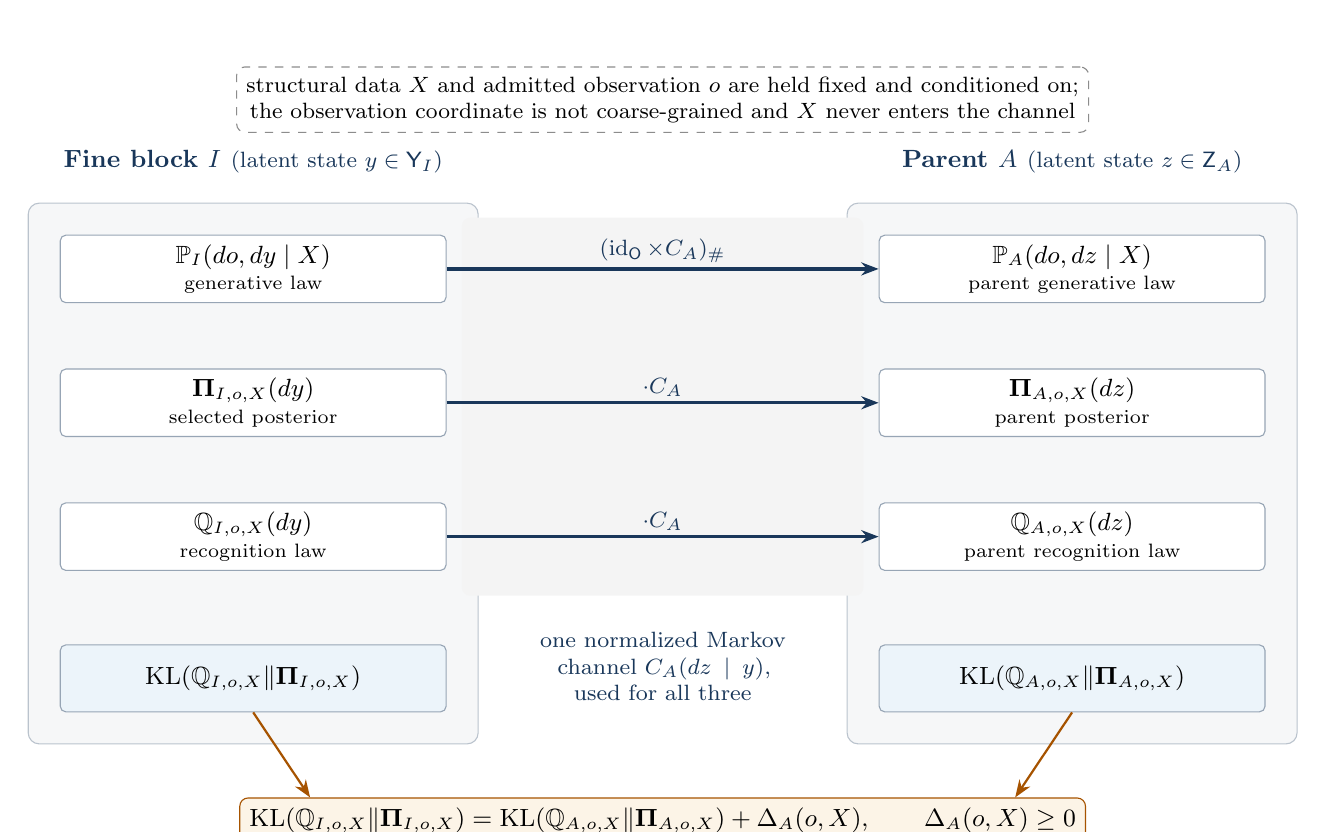
\begin{tikzpicture}[
  >={Stealth[length=2.2mm]},
  every node/.style={font=\small},
  law/.style={draw=deepblue!45, fill=white, rounded corners=2pt,
              minimum width=4.9cm, minimum height=8.5mm, align=center, font=\small},
  klbox/.style={draw=deepblue!45, fill=softblue, rounded corners=2pt,
                minimum width=4.9cm, minimum height=8.5mm, align=center, font=\small},
  panel/.style={draw=deepblue!30, fill=deepblue!4, rounded corners=4pt, inner sep=4mm},
  chan/.style={->, very thick, deepblue},
  clab/.style={font=\footnotesize, inner sep=1.5pt}
]
\def\LX{0}
\def\RX{10.4}
\fill[softgray, rounded corners=3pt] (2.65,-0.75) rectangle (7.75,4.05);
\node[law] (fP)  at (\LX, 3.4) {$\Prob_I(do,dy\mid X)$\\[-0.15em]{\scriptsize generative law}};
\node[law] (fPi) at (\LX, 1.7) {$\Post_{I,o,X}(dy)$\\[-0.15em]{\scriptsize selected posterior}};
\node[law] (fQ)  at (\LX, 0.0) {$\Rec_{I,o,X}(dy)$\\[-0.15em]{\scriptsize recognition law}};
\node[klbox] (fK) at (\LX,-1.8) {$\KL(\Rec_{I,o,X}\Vert\Post_{I,o,X})$};
\node[law] (pP)  at (\RX, 3.4) {$\Prob_A(do,dz\mid X)$\\[-0.15em]{\scriptsize parent generative law}};
\node[law] (pPi) at (\RX, 1.7) {$\Post_{A,o,X}(dz)$\\[-0.15em]{\scriptsize parent posterior}};
\node[law] (pQ)  at (\RX, 0.0) {$\Rec_{A,o,X}(dz)$\\[-0.15em]{\scriptsize parent recognition law}};
\node[klbox] (pK) at (\RX,-1.8) {$\KL(\Rec_{A,o,X}\Vert\Post_{A,o,X})$};
\begin{scope}[on background layer]
  \node[panel, fit=(fP)(fK)] (fpanel) {};
  \node[panel, fit=(pP)(pK)] (ppanel) {};
\end{scope}
\node[above=2.5mm of fpanel, font=\small\bfseries, deepblue]
  {Fine block $I$ \normalfont\footnotesize (latent state $y\in\mathsf Y_I$)};
\node[above=2.5mm of ppanel, font=\small\bfseries, deepblue]
  {Parent $A$ \normalfont\footnotesize (latent state $z\in\mathsf Z_A$)};
\draw[chan] (fP)  -- node[clab, above]{$(\id_{\mathsf O}\times C_A)_{\#}$} (pP);
\draw[chan] (fPi) -- node[clab, above]{$\cdot C_A$} (pPi);
\draw[chan] (fQ)  -- node[clab, above]{$\cdot C_A$} (pQ);
\node[align=center, font=\footnotesize, text=deepblue, text width=3.7cm] at (5.2,-1.65)
  {one normalized Markov channel $C_A(dz\mid y)$, used for all three};
\node[draw=orange!65!black, fill=softorange, rounded corners=3pt, align=center,
      font=\small, inner sep=3.5pt] (defect) at (5.2,-3.6)
  {$\KL(\Rec_{I,o,X}\Vert\Post_{I,o,X})
     =\KL(\Rec_{A,o,X}\Vert\Post_{A,o,X})+\Delta_A(o,X),
     \qquad \Delta_A(o,X)\geq 0$};
\draw[->, thick, orange!65!black] (fK.south) -- ($(defect.north west)+(0.9,0)$);
\draw[->, thick, orange!65!black] (pK.south) -- ($(defect.north east)+(-0.9,0)$);
\node[draw=black!45, fill=white, dashed, rounded corners=3pt, align=center,
      font=\footnotesize, inner sep=3.5pt] (ext) at (5.2,5.55)
  {structural data $X$ and admitted observation $o$ are held fixed and conditioned on;\\
   the observation coordinate is not coarse-grained and $X$ never enters the channel};
\end{tikzpicture}}
\caption{\textbf{The static coarse-graining step.} A fine block carries three laws: a generative law on observations and fine latents, a selected posterior version, and a recognition law. One normalized Markov channel \(C_A\) is applied to all three, acting on the latent coordinate only and leaving the observation coordinate and the structural data \(X\) untouched. The result is a parent triple of the same type. The forward relative entropy between recognition and posterior drops by exactly \(\Delta_A(o,X)\), the information the channel discarded.}
\label{fig:parent}
\end{figure}

\subsection{The declared fine objects}

Fix a finite nonempty block \(I\), a base point \(r_*\), structural data \(X\), and an admitted observation \(o\) with finite positive evidence density or mass \(p_X(o)\). The fine probabilistic datum consists of
\[
  \Prob_I(do,dy\mid X),
  \qquad
  \Post_{I,o,X}(dy),
  \qquad
  \Rec_{I,o,X}(dy).
\]
The generative law is fixed before recognition is chosen. The selected posterior is a measurable conditional version of the generative law. The recognition law is normalized, may be correlated across the child agents, and satisfies \(\Rec_{I,o,X}\ll\Post_{I,o,X}\) when a finite forward KL is required.

Three pieces of notation in that display deserve unpacking.

The \emph{structural data} \(X\) is the configuration the probabilistic machinery is set up on: the finite directed acyclic graph of agents with its edge set, the design incidence recording which agent is defined at which context, the geometric data such as the local frames and the graph links, and the parameters of the observation and transition mechanisms that are being held fixed for this pass. Loosely, \(X\) is the wiring diagram together with the knobs not currently being varied. Its defining property here is that it is external conditioning rather than a random variable. No kernel ever samples \(X\), and nothing ever integrates over it, so it appears as the same conditioning argument on both sides of every identity below. The parent inherits a coarser structural datum \(X_A=\chi_A(X)\) through a fixed measurable projection, and that too stays outside the channel. Keeping \(X\) outside is what allows the coarse-graining identity to be stated without giving \(X\) its own reference measure or normalizer.

The symbols \(do\) and \(dy\) are integrator notation, not derivatives. Writing \(\Prob_I(do,dy\mid X)\) names the joint measure on the product \(\mathsf O\times\mathsf Y_I\), with the two differentials recording which coordinate each infinitesimal cell belongs to, exactly as one writes \(\int f(x)P(dx)\) for a Lebesgue-Stieltjes integral. The reason for naming the measure rather than a density is that the statements below must remain valid when no density exists, and when the reference measures against which a density would be taken have not been declared.

The relation \(\Rec_{I,o,X}\ll\Post_{I,o,X}\) is absolute continuity: every set to which the posterior assigns zero mass is also assigned zero mass by the recognition law. Equivalently, the density \(d\Rec/d\Post\) exists. This is exactly the condition under which the forward relative entropy is defined by an integral at all, since
\[
  \KL(\Rec\Vert\Post)
  =\int\log\frac{d\Rec}{d\Post}d\Rec
  \quad\text{when }\Rec\ll\Post,
  \qquad\text{and }+\infty\text{ otherwise.}
\]
Without absolute continuity there is no Radon--Nikodym derivative whose logarithm could be integrated, and the convention assigns \(+\infty\). The failure is not a large finite penalty that could be traded against something else. If, for instance, the posterior is dominated by Lebesgue measure on \(\mathbb R^d\) while the recognition law is supported on a proper affine subspace, as happens when a recognition family ties several latents to one shared value, then the subspace carries posterior mass zero and recognition mass one, and the divergence is infinite outright. This is the mechanism that rules out degenerate recognition families, and it is why the hypothesis is carried explicitly rather than assumed away.

\subsection{One common coarse channel}

Let \(C_A(dz\mid y)\) be a normalized Markov channel from the fine latent state \(y\) to the parent state \(z\). It may be deterministic or stochastic. It may intentionally discard most microscopic information. The same \(C_A\) must act on recognition and posterior, while the observation and structural data remain outside the channel.

The parent objects are those in Equation~\eqref{eq:parent-triple}. This construction proves normalization, a selected parent posterior identity, and the appropriate absolute-continuity relation.

\subsection{The parent evaluator}
\label{sec:parent-evaluator}

The fine block came equipped with an evaluation map \(\ev_i\), which turned a model presentation into the generative kernel that presentation denotes. If the parent is to be an object of the same type rather than a bare law, it needs its own evaluator \(\ev_A:m_A\mapsto K_{A,m_A}^{X_A}\). The question is where that evaluator comes from, and the answer is that it need not be posited at all.

\emph{Disintegration} is the relevant tool. On standard Borel spaces, a joint probability law factors into a marginal on one group of coordinates together with a measurable family of conditional laws on the remaining coordinates, and that family is unique up to sets of marginal measure zero. This is the same theorem that produced the selected posterior version in Section~\ref{sec:four-objects}, applied along a different coordinate. Here it is applied to the pushed generative law \(\Prob_A=(\id_{\mathsf O}\times C_A)_{\#}\Prob_I\), disintegrated over the parent model and interface coordinates. What comes back is a measurable family of conditional laws over the remaining parent coordinates, including the observation, indexed by the parent model presentation. That family is precisely a kernel indexed by a presentation, which is to say an evaluation map, and it satisfies the compatibility identity
\[
  \Prob_A(\cdot\mid m_A,\xi_A,X)=K_{A,m_A}^{X_A}(\xi_A;\cdot)
\]
by construction rather than by assumption. This is the sense in which a parent evaluator is \emph{induced} from the pushed generative law by disintegration: the parent's mechanism is read off from the law the coarse channel already produced.

One may instead prefer to declare a parent evaluator by hand, typically because a convenient parametric form is wanted. That is permitted, but it comes with a debt: the declared family is admissible only when it agrees almost surely with the induced conditional kernel, and that agreement is a separate hypothesis which disintegration does not supply. The reason the condition cannot be dropped is that normalization and measurability do not pin down a mechanism. In the finite binary witness carried by the derivation package, the compatible evaluator is \(\ev_A(m)=K_m\) with \(K_m(B=1)=\tfrac14+\tfrac m2\), while the swapped family \(\ev_A'(m)=K_{1-m}\) is just as normalized and just as measurable, yet disagrees at both model points, each of which carries parent generative mass \(\tfrac12\). Nothing about being a well-formed Markov kernel distinguishes the two. Declaring the wrong one silently describes a different generative mechanism while every marginal still looks correct, which is exactly the failure mode that the almost-sure compatibility clause is there to exclude.

It is worth being equally clear about what disintegration does not do. It establishes existence of the induced tier. It does not validate an arbitrary predeclared evaluator, does not select the evaluator's extension over null sets canonically, does not make evaluation injective, and does not regularize a quotient of model presentations. Those remain the open obligations noted in Section~\ref{sec:ev}.

\begin{boundarybox}
The theorem constructs a full \emph{pointwise probabilistic datum}. It does not yet construct the local sections and gluing data required for a geometric agent over an overlap region. Calling the datum a meta-agent is law-level shorthand, not a proof of autonomous agency.
\end{boundarybox}

\subsection{Why marginals are insufficient}
\label{sec:marginals}

This subsection is the negative result that motivates everything above it, and it is worth saying plainly what work it does. There is a cheaper route to a parent, and it has to be closed off. The two-channel theorem of Section~\ref{sec:zero-distortion} already delivers a pair of consensus laws \((Q_q,Q_m)\), one for the belief channel and one for the model channel, under nothing more than zero transported distortion. It is tempting to declare that pair the meta-agent: the block agrees on what it believes, it agrees on what model it holds, and the effective description is the pair of agreements. The construction of Equation~\eqref{eq:parent-triple} is considerably more demanding, since it insists on pushing the entire correlated fine law through a single channel. If a pair of consensus marginals were already enough, that extra machinery would be unmotivated. The example below shows that it is not enough, which is precisely why the channel must act on the whole latent state at once rather than coordinate by coordinate. Historically this is also the gap between the earlier marginal-pair result and the later full-datum theorem recorded in Section~\ref{sec:provenance}.

Suppose two binary variables \(B\) and \(M\) are each fair. One joint law can put probability \(1/2\) on \((0,0)\) and \((1,1)\); another can put probability \(1/2\) on \((0,1)\) and \((1,0)\). Their \(B\)- and \(M\)-marginals are identical, but their correlations are opposite and their supports are disjoint. Therefore a parent belief law \(q_A^b\) and a parent model law \(q_A^m\) do not reconstruct the full parent law.

The failure is as large as it can be. Because the two joint laws have disjoint supports, neither is absolutely continuous with respect to the other, so both directed relative entropies between them are \(+\infty\) even though every displayed marginal matches exactly. Marginal agreement is therefore compatible with maximal joint disagreement, and no refinement of the marginal statement can recover the difference.

This distinction matters physically. A university can discard most microscopic details about students and faculty while retaining organization-level variables. That lossy parent can still be well-defined, but its joint law must be constructed by a coarse channel. It cannot be inferred from a list of separate consensus marginals.

\section{The exact information cost of coarse graining}
\label{sec:info-cost}

\subsection{Relative-entropy chain rule}

Disintegrate the fine recognition and posterior laws over the parent state \(z\):
\[
  \widehat{\Rec}_{I,o,X}(dy\mid z),
  \qquad
  \widehat{\Post}_{I,o,X}(dy\mid z).
\]
The instruction in that sentence is worth reading slowly, because it is where the defect term comes from. The channel is many to one: a whole set of fine states \(y\) is mapped to the same parent state \(z\), and that set is the \emph{fiber} over \(z\). Knowing \(z\) therefore tells you which fiber you are in but nothing about where in the fiber you are. Disintegration splits each of the two fine laws accordingly, into a marginal over parent states and a family of conditional laws inside the fibers. The hatted objects \(\widehat{\Rec}_{I,o,X}(dy\mid z)\) and \(\widehat{\Post}_{I,o,X}(dy\mid z)\) are exactly those within-fiber conditionals: they say how recognition mass and posterior mass are respectively distributed among the fine states that the parent cannot tell apart. Figure~\ref{fig:disintegration} shows the picture.

\begin{figure}[ht]
\centering
\resizebox{\textwidth}{!}{%
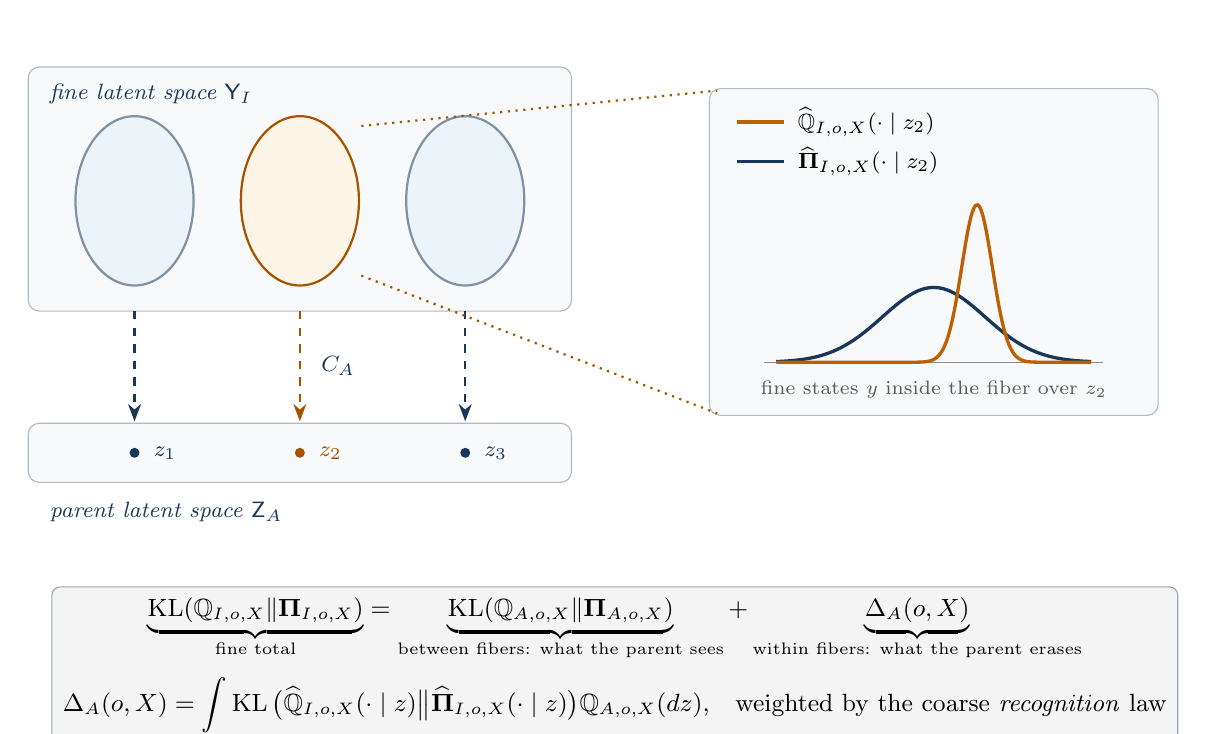
\begin{tikzpicture}[
  >={Stealth[length=2.2mm]},
  every node/.style={font=\small},
  fiberstyle/.style={draw=deepblue!55, fill=softblue, thick},
  frame/.style={draw=deepblue!35, fill=deepblue!3, rounded corners=4pt}
]
\node[frame, minimum width=6.9cm, minimum height=3.1cm] (Ybox) at (3.4,3.1) {};
\node[anchor=north west, font=\footnotesize\itshape, text=deepblue]
  at (0.1,4.55) {fine latent space $\mathsf Y_I$};
\node[fiberstyle, ellipse, minimum width=1.5cm, minimum height=2.15cm] (f1) at (1.3,2.95) {};
\node[fiberstyle, ellipse, minimum width=1.5cm, minimum height=2.15cm, fill=softorange,
      draw=orange!65!black] (f2) at (3.4,2.95) {};
\node[fiberstyle, ellipse, minimum width=1.5cm, minimum height=2.15cm] (f3) at (5.5,2.95) {};
\node[frame, minimum width=6.9cm, minimum height=0.75cm] (Zbox) at (3.4,-0.25) {};
\node[anchor=north west, font=\footnotesize\itshape, text=deepblue]
  at (0.1,-0.75) {parent latent space $\mathsf Z_A$};
\foreach \x/\lab/\col in {1.3/{z_1}/deepblue, 3.4/{z_2}/{orange!65!black}, 5.5/{z_3}/deepblue}{
  \fill[\col] (\x,-0.25) circle (1.8pt);
  \node[font=\footnotesize, text=\col, right=1.2mm] at (\x,-0.25) {$\lab$};
}
\draw[->, thick, deepblue, dashed] (1.3,1.55) -- (1.3,0.15);
\draw[->, thick, orange!65!black, dashed] (3.4,1.55) -- (3.4,0.15);
\draw[->, thick, deepblue, dashed] (5.5,1.55) -- (5.5,0.15);
\node[font=\footnotesize, text=deepblue, right=0.5mm] at (3.5,0.85) {$C_A$};
\begin{scope}[shift={(8.6,0)}]
  \node[frame, minimum width=5.7cm, minimum height=4.15cm] at (2.85,2.3) {};
  \draw[very thick, orange!75!black] (0.35,3.95) -- (0.95,3.95);
  \node[right, font=\footnotesize] at (1.0,3.95) {$\widehat{\Rec}_{I,o,X}(\cdot\mid z_2)$};
  \draw[very thick, deepblue] (0.35,3.45) -- (0.95,3.45);
  \node[right, font=\footnotesize] at (1.0,3.45) {$\widehat{\Post}_{I,o,X}(\cdot\mid z_2)$};
  \begin{scope}[shift={(2.85,0.9)}]
    \draw[black!45] (-2.15,0) -- (2.15,0);
    \draw[very thick, deepblue, smooth, samples=90, domain=-2.0:2.0]
      plot (\x, {0.95*exp(-\x*\x/0.85)});
    \draw[very thick, orange!75!black, smooth, samples=140, domain=-2.0:2.0]
      plot (\x, {2.0*exp(-(\x-0.55)*(\x-0.55)/0.075)});
  \end{scope}
  \node[font=\scriptsize, text=black!65] at (2.85,0.55)
    {fine states $y$ inside the fiber over $z_2$};
\end{scope}
\draw[dotted, thick, orange!65!black] (4.18,3.9) -- (8.7,4.35);
\draw[dotted, thick, orange!65!black] (4.18,2.0) -- (8.7,0.25);
\node[draw=deepblue!45, fill=softgray, rounded corners=3pt, align=center,
      inner sep=4pt, font=\small] at (7.4,-2.95)
  {$\underbrace{\KL(\Rec_{I,o,X}\Vert\Post_{I,o,X})}_{\text{fine total}}
    =\underbrace{\KL(\Rec_{A,o,X}\Vert\Post_{A,o,X})}_{\text{between fibers: what the parent sees}}
    +\underbrace{\Delta_A(o,X)}_{\text{within fibers: what the parent erases}}$\\[0.55em]
   $\Delta_A(o,X)=\displaystyle\int\KL\big(\widehat{\Rec}_{I,o,X}(\cdot\mid z)\big\Vert
     \widehat{\Post}_{I,o,X}(\cdot\mid z)\big)\Rec_{A,o,X}(dz)$,
   \ \ weighted by the coarse \emph{recognition} law};
\end{tikzpicture}}
\caption{\textbf{Disintegration over the parent state.} The coarse channel is many to one, so each parent state \(z\) labels a fiber of fine states that the parent cannot distinguish. Disintegrating the fine recognition and posterior laws over \(z\) separates a between-fiber part, which the parent still sees, from a within-fiber part, which it erases. The blow-up shows one fiber in which recognition is sharp and the posterior is broad: the parent-level laws can agree exactly while a large disagreement survives inside the fiber. The figure draws a deterministic channel for clarity; for a stochastic channel the fibers are replaced by the conditional laws \(C_A(\cdot\mid y)\) and the same decomposition holds.}
\label{fig:disintegration}
\end{figure}

The discarded-information defect is
\begin{equation}
  \Delta_A(o,X)
  =
  \int
  \KL\left(
  \widehat{\Rec}_{I,o,X}(\cdot\mid z)
  \Vert
  \widehat{\Post}_{I,o,X}(\cdot\mid z)
  \right)
  \Rec_{A,o,X}(dz).
  \label{eq:defect}
\end{equation}
The weighting measure is the coarse recognition law, not an arbitrary reference law, and this is forced rather than chosen. Relative entropy is by definition an expectation taken under its left argument, so any exact decomposition of \(\KL(\Rec_{I,o,X}\Vert\Post_{I,o,X})\) must average the fiberwise term against the parent-state image of the recognition law, which is \(\Rec_{A,o,X}\). Substituting the parent posterior \(\Post_{A,o,X}\) as the weight yields a different number that does not sum back to the fine divergence, so the identity below fails outright rather than degrading. Standard-Borel disintegration gives the additive identity
\begin{equation}
  \KL(\Rec_{I,o,X}\Vert\Post_{I,o,X})
  =
  \KL(\Rec_{A,o,X}\Vert\Post_{A,o,X})
  +\Delta_A(o,X)
  \label{eq:kl-chain}
\end{equation}
in the extended nonnegative reals.

The physical content is straightforward. The first term on the right is the mismatch visible to the parent. The second is the mismatch still present among fine states that the parent regards as the same state. Coarse graining cannot increase the visible KL divergence; the missing amount is exactly \(\Delta_A\).

\subsection{Variational free energy}

At fixed evidence, define
\begin{equation}
  \mathcal F_I(o,X)
  =
  \KL(\Rec_{I,o,X}\Vert\Post_{I,o,X})
  -\log p_X(o),
  \label{eq:fine-vfe}
\end{equation}
with the analogous definition for \(\mathcal F_A\). Since the observation coordinate and its evidence are unchanged, the same finite real number \(-\log p_X(o)\) is added to both KL terms. Hence
\begin{equation}
  \mathcal F_I(o,X)
  =
  \mathcal F_A(o,X)+\Delta_A(o,X)
  \label{eq:vfe-chain}
\end{equation}
as an extended-real identity.

A continuous evidence density can exceed one, so a finite VFE can be negative. Only the KL terms and \(\Delta_A\) live in \([0,+\infty]\). If the fine KL is finite, ordinary subtraction is valid:
\[
  \mathcal F_I-\mathcal F_A=\Delta_A.
\]
Without that finiteness premise, the expression \(+\infty-(+\infty)\) is undefined. A bare equality \(+\infty=+\infty\) implies neither zero discarded information nor recovery.

The zero-defect criterion itself is sharper. Regardless of whether the total KL is finite,
\begin{equation}
  \Delta_A(o,X)=0
  \quad\Longleftrightarrow\quad
  \widehat{\Rec}_{I,o,X}(\cdot\mid z)
  =
  \widehat{\Post}_{I,o,X}(\cdot\mid z)
  \quad
  \Rec_{A,o,X}\text{-almost surely}.
  \label{eq:zero-defect}
\end{equation}
Thus the coarse state is sufficient for this recognition-posterior pair exactly when the discarded conditional laws agree.

\begin{boundarybox}
\(\Delta_A\) is an information-theoretic loss term. Calling it thermodynamic entropy production would require an additional physical model, time evolution, and identification of thermodynamic variables. The static theorem does not make that identification.
\end{boundarybox}

\section{A worked binary example}

Let the fine latent state be \(Y=(M,B,E)\), with all three variables binary, and let the observation space contain one admitted value. The model bit is fair:
\[
  \Pr(M=0)=\Pr(M=1)=\frac12.
\]
Given \(M=m\), let
\[
  \Pr(B=1\mid M=m)=\frac14+\frac{m}{2}.
\]
Thus \(B\) tends to agree with \(M\). In the posterior, let \(E\) be an independent fair bit. The posterior marginal on \((M,B)\), displayed in the order \((M,B)\), is
\begin{center}
\begin{tabular}{ccccc}
\toprule
\((M,B)\) & \((0,0)\) & \((0,1)\) & \((1,0)\) & \((1,1)\) \\
\midrule
\(\Post_{I}(M,B)\) & \(3/8\) & \(1/8\) & \(1/8\) & \(3/8\) \\
\bottomrule
\end{tabular}
\end{center}
Each cell is split equally between \(E=0\) and \(E=1\).

Choose a recognition law with the same \((M,B)\) marginal but impose \(E=B\) exactly. On the support of the recognition law, the density ratio \(d\Rec_I/d\Post_I\) equals \(2\). Therefore
\[
  \KL(\Rec_I\Vert\Post_I)=\log 2.
\]
Now let the coarse channel retain \((M,B)\) and discard \(E\). Since the two laws have the same retained marginal,
\[
  \Rec_A=\Post_A,
  \qquad
  \KL(\Rec_A\Vert\Post_A)=0.
\]
Conditioned on a parent state \((m,b)\), recognition assigns \(E=b\) with certainty while the posterior keeps \(E\) fair. Every conditional KL is \(\log 2\), so
\[
  \Delta_A=\log 2.
\]
The chain rule reads
\[
  \log 2=0+\log 2.
\]

\begin{physicalreading}
The parent is exact about everything it retains and blind to the entire recognition-posterior disagreement. This is not a failure of the theorem. It is what the defect term is designed to expose.
\end{physicalreading}

\section{Forward-KL parents and approximate agreement}

\subsection{The unrestricted forward-KL barycenter}
\label{sec:barycenter}

Transport full laws \(P_i=(T_{\gamma_i})_{\#}p_i\) into one root frame, as in Section~\ref{sec:zero-distortion}, and choose positive weights \(w_i\) summing to one. Their mixture
\[
  M=\sum_i w_iP_i
\]
satisfies
\begin{equation}
  \sum_iw_i\KL(P_i\Vert Q)
  =
  \sum_iw_i\KL(P_i\Vert M)
  +\KL(M\Vert Q)
  \label{eq:barycenter}
\end{equation}
for every comparison law \(Q\), with the extended support convention.

A \emph{comparison law} is simply a candidate parent: any normalized law on the root frame's state space that one might propose as the block's effective description, and against which each child's transported law is then scored. It is the free variable of the optimization rather than a distinguished object, which is why the identity is asserted for every \(Q\) rather than for a particular one. The content of Equation~\eqref{eq:barycenter} is that the candidate appears on the right-hand side only inside the single nonnegative term \(\KL(M\Vert Q)\), which vanishes exactly when \(Q=M\). The mixture is therefore the unique minimizer of the averaged forward-KL objective over all candidates, with no restriction to any parametric family. The extended support convention is what makes this unconditional: relative entropy is \(+\infty\) when absolute continuity fails, and under that convention both sides are simultaneously \(+\infty\) whenever some child law is singular against the candidate.

The zero-distortion case of Section~\ref{sec:zero-distortion} is the degenerate instance of the same statement. There the transported laws all coincide, so the mixture equals their common value and \(M=Q_x\). The root law of Equation~\eqref{eq:root-law} is the barycenter of a family whose members already agree.

This is a mixture law, not a product of experts and not precision pooling. Gaussian precision formulas arise only after imposing a restricted Gaussian family or changing the orientation of the optimization. They are useful computational charts, not the general parent theorem.

\subsection{Small distortion}
\label{sec:small-distortion}

The theorem of Section~\ref{sec:zero-distortion} is an exact equivalence at \(\mathcal D_x=0\), and that is why this subsection is needed. No real network sits exactly at zero distortion. Without a statement about small but nonzero \(\mathcal D_x\), the zero-distortion theorem would be a knife-edge result: perfectly sharp on a set of measure zero in parameter space and silent one step away from it. What follows is what turns it into a statement about a neighborhood.

The obstacle is that relative entropy is not a metric. It is asymmetric and it obeys no triangle inequality, so knowing that every edge term is small does not by itself bound the disagreement between two nodes many hops apart; there is no legitimate way to add edge divergences along a path. Pinsker's inequality provides the exit by converting each edge estimate into total variation,
\[
  \|P-P'\|_{\mathrm{TV}}
  \leq
  \sqrt{\tfrac12\KL(P\Vert P')},
\]
and total variation is a genuine metric.

The bound is then assembled as follows. Fix a rooted spanning tree \(T_x\), let \(\eta_{\min}^x\) be the smallest edge-event weight carried by a tree edge, and let \(d_x\) be the diameter of the tree. Suppose \(\mathcal D_x\leq\varepsilon_x\). Because \(\mathcal D_x\) is a sum of nonnegative terms \(\eta_{ij}^x\KL(\cdot\Vert\cdot)\), no single tree-edge divergence can exceed \(\varepsilon_x/\eta_{\min}^x\), and Pinsker converts that into one uniform per-edge total-variation bound
\[
  \delta_x=\sqrt{\frac{\varepsilon_x}{2\eta_{\min}^x}}.
\]
Chaining along the unique tree path between two nodes with the triangle inequality gives
\[
  \|P_u^x-P_v^x\|_{\mathrm{TV}}
  \leq
  \operatorname{dist}_{T_x}(u,v)\delta_x
  \leq
  d_x\delta_x,
\]
and convexity of total variation extends the same bound to the distance between any transported node law and the mixture.

Two costs are worth stating plainly. The bound accumulates linearly in graph distance, so it is weakest exactly for the most distant pairs, and the factor \(1/\eta_{\min}^x\) means that a single rarely used edge with small occupancy weight degrades it. It also depends on which spanning tree was chosen, so a different tree yields a different valid constant rather than a canonical one. The result is an approximate agreement statement in total variation, not a claim that KL itself is a path metric.

\section{Coarse-graining the network}
\label{sec:network}

The node laws and the interaction network must both be coarse-grained. Figure~\ref{fig:network} shows the network half of the step.

\begin{figure}[ht]
\centering
\resizebox{\textwidth}{!}{%
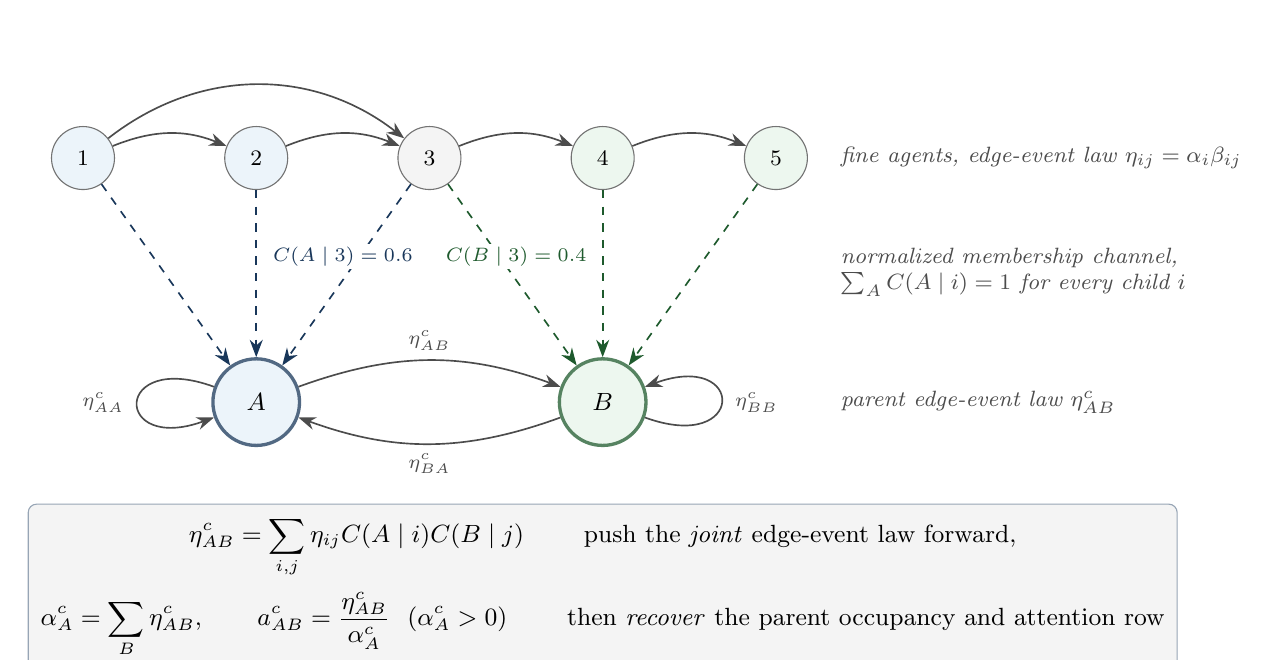
\begin{tikzpicture}[
  >={Stealth[length=2.2mm]},
  every node/.style={font=\small},
  ch/.style={draw=black!55, circle, minimum size=8mm, inner sep=0pt, font=\footnotesize},
  par/.style={draw, circle, minimum size=11mm, inner sep=0pt, font=\small, very thick},
  ed/.style={->, semithick, black!70},
  mem/.style={->, dashed, semithick}
]
\foreach \i/\x/\col in {1/0/softblue, 2/2.2/softblue, 3/4.4/softgray,
                        4/6.6/softgreen, 5/8.8/softgreen}
  \node[ch, fill=\col] (n\i) at (\x,3.7) {$\i$};
\node[par, fill=softblue,  draw=deepblue!75] (A) at (2.2,0.6) {$A$};
\node[par, fill=softgreen, draw=deepgreen!75] (B) at (6.6,0.6) {$B$};
\foreach \a/\b/\bd in {1/2/22, 2/3/22, 3/4/22, 4/5/22, 1/3/38}
  \draw[ed] (n\a) to[bend left=\bd] (n\b);
\node[anchor=west, font=\footnotesize\itshape, text=black!70] at (9.5,3.7)
  {fine agents, edge-event law $\eta_{ij}=\alpha_i\beta_{ij}$};
\foreach \i in {1,2} \draw[mem, deepblue]  (n\i) -- (A);
\foreach \i in {4,5} \draw[mem, deepgreen] (n\i) -- (B);
\draw[mem, deepblue]  (n3) -- (A);
\draw[mem, deepgreen] (n3) -- (B);
\node[font=\scriptsize, text=deepblue,  fill=white, inner sep=1pt] at (3.30,2.45) {$C(A\mid 3)=0.6$};
\node[font=\scriptsize, text=deepgreen, fill=white, inner sep=1pt] at (5.50,2.45) {$C(B\mid 3)=0.4$};
\node[anchor=west, font=\footnotesize\itshape, text=black!70, align=left] at (9.5,2.25)
  {normalized membership channel,\\ $\sum_A C(A\mid i)=1$ for every child $i$};
\draw[ed] (A) to[bend left=20] node[font=\scriptsize, above]{$\eta^{c}_{AB}$} (B);
\draw[ed] (B) to[bend left=20] node[font=\scriptsize, below]{$\eta^{c}_{BA}$} (A);
\draw[ed] (A) to[out=160,in=200,looseness=9]
  node[font=\scriptsize, left=0.5mm]{$\eta^{c}_{AA}$} (A);
\draw[ed] (B) to[out=340,in=20,looseness=9]
  node[font=\scriptsize, right=0.5mm]{$\eta^{c}_{BB}$} (B);
\node[anchor=west, font=\footnotesize\itshape, text=black!70] at (9.5,0.6)
  {parent edge-event law $\eta^{c}_{AB}$};
\node[draw=deepblue!45, fill=softgray, rounded corners=3pt, align=center,
      inner sep=4.5pt, font=\small] at (6.6,-1.75)
  {$\displaystyle \eta^{c}_{AB}=\sum_{i,j}\eta_{ij}C(A\mid i)C(B\mid j)$
    \qquad push the \emph{joint} edge-event law forward,\\[0.45em]
   $\displaystyle \alpha^{c}_{A}=\sum_{B}\eta^{c}_{AB},
    \qquad a^{c}_{AB}=\frac{\eta^{c}_{AB}}{\alpha^{c}_{A}}\ \ (\alpha^{c}_{A}>0)$
    \qquad then \emph{recover} the parent occupancy and attention row};
\end{tikzpicture}}
\caption{\textbf{Coarse-graining the interaction network.} Children are assigned to parents by a normalized membership channel, which may be soft: child \(3\) belongs to \(A\) with weight \(0.6\) and to \(B\) with weight \(0.4\), and its memberships sum to one so no mass is duplicated. The object pushed forward is the joint edge-event law \(\eta_{ij}\), not the conditional attention row. The parent receiver occupancy and the parent attention row are then recovered from the pushed joint by disintegration.}
\label{fig:network}
\end{figure}

\subsection{The membership channel}

A \emph{normalized membership channel} \(C(A\mid i)\) is a Markov kernel from the child index to the parent label: the weights are nonnegative and satisfy \(\sum_A C(A\mid i)=1\) for every child \(i\). It answers the question ``which parent does child \(i\) belong to'' probabilistically rather than categorically. A hard partition is the deterministic special case, in which each child has exactly one parent and the weight is an indicator. A normalized soft membership permits several nonzero memberships for one child provided they sum to one, so a child can be split between parents without any probability mass being duplicated.

The contrast worth keeping in view is with a literal replicated cover, which assigns each child a unit membership to every parent whose region contains it. Its columns then sum to more than one, so it is not a Markov channel at all. It records multiplicity rather than a distribution, and treating it as if it were a channel double counts both mass and joint edge-event contributions. Coverings of this kind are perfectly reasonable objects; they simply carry different mass semantics and cannot be substituted into the pushforward below.

\subsection{Why the joint edge-event law is what pushes forward}

If \(C(A\mid i)\) is a normalized membership channel, the correct scalar network object to push forward is the joint edge-event law \(\eta_{ij}\), not only the conditional attention row. A deterministic endpoint assignment gives
\[
  \eta_{AB}^{c}
  =
  \sum_{i,j}
  \eta_{ij}
  C(A\mid i)C(B\mid j).
\]
The parent receiver occupancy and conditional row are recovered by
\[
  \alpha_A^c=\sum_B\eta_{AB}^c,
  \qquad
  a_{AB}^c=\frac{\eta_{AB}^c}{\alpha_A^c}
\]
when \(\alpha_A^c>0\).

The reason is a type mismatch rather than a matter of taste. A row-stochastic matrix \(\beta_{ij}\) is a conditional law of the source given the receiver: each row separately sums to one, so the whole array sums to the number of receivers rather than to one. It is a kernel, not a measure on the edge set, and a kernel is not the kind of object that can be pushed through a coarse-graining map on its own. Multiplying by the receiver occupancy \(\alpha_i\) supplies the missing mass and turns the kernel into the genuine joint measure \(\eta_{ij}\), which sums to one over all directed edges. That measure can be pushed forward through any declared endpoint kernel, and the coarse conditional row is then \emph{recovered} by disintegration rather than defined by fiat. The order of operations matters: push the joint, then condition.

The cost of getting the order wrong is not subtle. Take two receivers merged into one parent \(A\), with source blocks \(B_1\) and \(B_2\), occupancies \(\alpha_1=0.9\) and \(\alpha_2=0.1\), and rows \(\beta_1=(0.5,0,0.3,0.2)\) and \(\beta_2=(0,0,0,1)\) over four sources of which the first two lie in \(B_1\). Pushing the joint and then conditioning gives the parent row \((0.45,0.55)\). Averaging the two attention rows directly gives \((0.25,0.75)\). The discrepancy is not rounding; it arises because row averaging silently assumes uniform receiver occupancy, and here the second receiver, which routes all of its weight to \(B_2\), fires only a ninth as often as the first. The joint law knows this and the conditional row does not.

\subsection{Marked and gauge-valued edges}

Everything above concerns scalar weights. Edges in this theory can also carry a group element, namely the transport attached to them, and for those the same recipe fails. Averaging matrices is generally unsafe because the average can leave the group: the arithmetic mean of the two planar rotations by \(+\pi/2\) and \(-\pi/2\) is the zero matrix, which is neither a rotation nor even invertible. The general point is that \(\mathrm{GL}(K)\) and its compact subgroups are not convex, so a convex combination of legitimate transports need not be a legitimate transport at all.

The exact closure therefore retains three kinds of mark rather than averaging them away. The \emph{conditional boundary marks} are the dressed transports attached to edges crossing a block boundary, each raw edge transport re-expressed in the two blocks' chosen root frames, which is what allows a parent-level edge to still be composed with other parent-level edges. The \emph{connected-component labels} record that a block whose internal positive-support graph is disconnected splits into several components, each carrying its own parent index and its own root; a disconnected block is not silently collapsed to a single node, because nothing asserts any transport between its components and so nothing says how their frames should be compared. The \emph{internal based holonomy} is the representation of the block's internal loop group at its chosen root, recording which internal loops fail to close and how.

The closing sentence, that erasing those marks requires another declared coarse channel and another theorem, means the following. Collapsing several components onto one root, or replacing a family of boundary transports by a single summary transport, is not a bookkeeping simplification. It is itself a coarse-graining step, performed on the mark fibers rather than on the state fibers, and it therefore needs the same two things every coarse-graining step in this document has needed: a declared normalized channel saying exactly how the marks are to be merged, and a proof that the merge is consistent with the structure that survives. Quotienting each holonomy separately does not suffice, because doing so loses the orientation of each holonomy relative to the root features and the boundary legs, which is precisely the information that made the marks worth retaining. No such theorem exists here. It sits on the open list of Section~\ref{sec:status}, where the nearest scoped statement asks for a canonical minimal compression and a characterization of when a family of marks compresses to one invertible transporter with one weight.

\section{Interventions and passive agreement}

\subsection{What an intervention is}
\label{sec:intervention}

One point should be made before the definition, because it explains the odd grammar of the sentence that follows. The comparison theorem does not yet exist. It is the first entry on the open list of Section~\ref{sec:status} and the first of the three next steps in Section~\ref{sec:next-steps}. What this subsection fixes is the vocabulary that theorem will be stated in, so the reader is being handed a definition in advance of the result it is for.

In that setting, an intervention is an analyst-declared probe of a mechanism. Consider a typed chain
\[
  R\longrightarrow E\longrightarrow O,
\]
where \(R\) is a retained input or parameter, \(E\) is an internal mediator, and \(O\) is a retained output or observation. An intervention replaces the ordinary mechanism feeding \(E\) with a declared preparation law while leaving the retained boundary roles fixed. One then asks how the distribution of \(O\) responds.

Unpacking that: ``analyst-declared'' means the intervention is not something the system does. It is an operation performed on the description. One takes the model, deletes the factor that would ordinarily generate \(E\) from its parents, substitutes a distribution of one's own choosing, and recomputes. The substituted distribution is the \emph{declared preparation law}. When it is a point mass, the operation is exactly Pearl's \(\mathrm{do}(E=e)\); when it is an arbitrary normalized kernel drawn from a declared admissible set, the operation is the softer variant this theory actually uses. ``Typed'' means that \(R\), \(E\), and \(O\) are roles rather than merely variables: the role labels are part of the object, and any morphism or comparison admitted between two such chains is required to preserve them. That is the sense in which the ``retained boundary roles'' stay fixed, namely that the ordered pair \((R,O)\) keeps its identity across every comparison, whatever happens at \(E\).

The reason this apparatus is worth the trouble is that passive data genuinely underdetermines mechanism, and the theory carries an explicit finite witness of the fact. Let \(R\) be a fair bit and let each arrow be a binary symmetric channel, so that \(E\) flips \(R\) with probability \(a\) and \(O\) flips \(E\) with probability \(b\). Compare the chain with \((a,b)=(\tfrac14,\tfrac13)\) against the chain with \((a,b)=(\tfrac13,\tfrac14)\). Their retained \((R,O)\) laws are identical, both equal to \((\tfrac{7}{24},\tfrac{5}{24},\tfrac{5}{24},\tfrac{7}{24})\) in the order \((0,0),(0,1),(1,0),(1,1)\), because the passive law depends on \(a\) and \(b\) only through the symmetric combination \((1-a)(1-b)+ab\). No amount of passive observation separates them. Now probe. Setting \(E=0\) gives \((\tfrac13,\tfrac16,\tfrac13,\tfrac16)\) for the first chain and \((\tfrac38,\tfrac18,\tfrac38,\tfrac18)\) for the second, and the first of these vectors does not appear anywhere in the second chain's complete response image under the admitted boundary relabelings. The two mechanisms are therefore provably distinguishable by intervention and provably indistinguishable without it.

This use of intervention does not assert that actions, plans, or controls are primitive ingredients of reality. It is a mathematical way to distinguish mechanisms that look identical when left alone.

\begin{translationbox}
The symbol \(R\) is not being reused from Section~\ref{sec:barycenter}. There, the comparison law was a candidate parent law and is written \(Q\). Here, \(R\) is the retained input node of the intervention chain, which is the notation the canonical sources use for that role throughout.
\end{translationbox}

\subsection{Passive agreement}

Two mechanisms passively agree when they give the same retained \((R,O)\) law in the unperturbed experiment. They need not have the same full joint law on \((R,E,O)\). If an intervention at \(E\) produces different retained output laws, the passive data hid a mechanistic difference.

\begin{physicalreading}
The analogy is two materials with the same equilibrium equation of state but different response functions. Passive agreement records the shared unforced behavior. The intervention probes susceptibility.
\end{physicalreading}

Why specify the comparison rules so carefully? If one is allowed to erase the mediator target, swap input and output, reverse time, or choose a different relabeling for every protocol, one is no longer testing the same mechanistic equivalence. Those moves may define useful comparison problems, but they are different problems. A theorem that varies these admissible morphisms remains a downstream task.

\section{Static closure is not dynamics or agency}

\subsection{The moving-map defect}

Suppose a fine state obeys a declared dynamics
\[
  \dot y=V_t(y)
\]
and a possibly moving deterministic coarse map is \(c_t\). The coarse state \(z=c_t(y)\) obeys
\[
  \dot z
  =
  \partial_t c_t(y)+Dc_t(y)V_t(y).
\]
Exact trajectory semiconjugacy to a proposed coarse vector field \(\overline V_t\) requires
\begin{equation}
  \delta_t
  =
  \partial_t c_t+Dc_tV_t-\overline V_t\circ c_t
  =
  0.
  \label{eq:semiconjugacy}
\end{equation}
This is an additional dynamical statement. It does not follow from the static pushforward theorem. The term \(\partial_t c_t\) is present whenever the coarse map or membership changes.

Autonomy requires more than Equation~\eqref{eq:semiconjugacy}: the relevant fields and maps must have the appropriate time independence or closed state dependence, and the resulting flow must be well posed. Sustained nonequilibrium requires a source of circulating or driven behavior, such as open boundary flux, stochastic driving, an antisymmetric sector, adaptive coarse maps, or a proved cross-scale feedback mechanism. Frozen dissipative gradient flow will generally relax toward an equilibrium sector.

\subsection{Where Wheelerian participation could enter}

The present theorem maps fine probabilistic structure upward to a parent description. A participatory theory would also let emergent coarse variables modify the fine dynamics that sustain them. Such a loop could support nonequilibrium evolution, but it must be derived from a typed coupled action or a controlled reduction. Fine-to-coarse influence plus an independently added coarse-to-fine force risks double counting.

The program therefore leaves Wheelerian feedback as a concrete open direction rather than treating it as a consequence of static coarse graining. The same caution applies to emergent agency. Universal variational evolution and autonomous goal-directed behavior are different claims.

\subsection{No unique microscopic physics is assumed}

The construction does not require every scale to share one literal generative model or one unique latent DAG. A bacterium, a human, and a university can occupy different model spaces and carry different laws over model presentations. What is shared across a successful coarse-graining step is a typed relation between fine and parent probabilistic objects, not one privileged ontology.

This allows a constructivist reading: each scale has an effective ``physics'' encoded by its generative regularities. The theory can still produce invariant consequences, such as information-loss identities, holonomy constraints, and induced pullback geometry. It does not thereby derive a unique underlying microscopic world model.

\section{What has been proved, what is conditional, and what remains open}
\label{sec:status}

\begin{table}[ht]
\centering
\small
\begin{tabularx}{\textwidth}{>{\raggedright\arraybackslash}p{0.16\textwidth}X}
\toprule
\textbf{Status} & \textbf{Content} \\
\midrule
Established &
At one fixed \(r_*\), \(X\), and admitted \(o\): normalized parent \(\Prob_A\), \(\Rec_{A,o,X}\), and \(\Post_{A,o,X}\); induced or explicitly compatible parent evaluation; derived marginal projection identities; the extended KL/VFE chain; the exact zero-defect criterion; finite pairwise recovery results; zero transported-distortion theorem; forward-KL mixture parent; normalized network pushforward; and explicit finite counterexamples to common shortcuts. \\
\addlinespace
Conditional &
Holonomy blindness requires declared full-law actions, compatible posterior versions, channel equivariance, evaluator covariance, and the appropriate fixed-\((o,X)\) stabilizer. Compact continuous holonomy averaging needs domination and integrability assumptions. Gaussian stability results apply only in their declared finite realization. \\
\addlinespace
Diagnostic &
Spectral gaps, finite KL thresholds, symbolic checks, and numerical experiments can test a proposed construction; the 2026-08-17 rescaling-map measurements of Section~\ref{sec:rescaling-measured} are of this kind: exact covariance and holonomy-conservation checks passed, the compatibility law refuted at its pre-registered tolerance, and per-ratio contraction onto factorized, ratio-typed fixed structures. They do not select the coarse channel or prove a universal theorem. \\
\addlinespace
Open &
A comparison-category theorem; extension across \(\mathcal U_A\); local sections and gluing; changing active sets; canonical channel, membership, and partition selection; geometric meta-agents; autonomous agency; nonequilibrium persistence; physical time; continuum limits; unique microscopic physics; ontology; adaptive attention dynamics; nonlinear full-law dynamical closure; whether the measured composition defect contracts on deeper flows; and which boundary-multiplicity architectures sustain interacting fixed structures. \\
\bottomrule
\end{tabularx}
\caption{The current boundary of the theory.}
\label{tab:status}
\end{table}

\subsection{How the certification is recorded}

The box below quotes a hash, and a reader meeting it cold is entitled to ask what it is doing in a physics guide. The theory program freezes each completed result as a release package. The frozen statement of the problem, called the target, is serialized to canonical JSON with sorted keys and no whitespace, and the SHA-256 digest of that serialization becomes the package identifier. Quoting the digest is how a document names the exact statement it is claiming rather than an informal paraphrase of it: change one word of the target statement and the digest changes, so a claim that cites a digest can be checked against the frozen text instead of being argued about. The digest below is reproducible from this repository by hashing the canonical serialization of the target object in the package's problem contract.

The target itself is a mixed-quantifier conjunction. Its affirmative half asserts, for every declared standard-Borel fine and parent datum meeting the frozen premises, that the full normalized pointwise parent datum can be constructed through one normalized recognition-independent channel, that the parent posterior and recognition laws and their projection identities follow, that the exact chain identity holds with a nonnegative conditional-KL defect and the stated equality criterion, and that exactly one declared full-law holonomy alternative is established. Its negative half requires in-domain counterexamples against five shortcuts: that marginals determine a full parent law, that split-channel VFE identities hold unconditionally, that model-marginal agreement suffices for evaluation compatibility, that trivial holonomy suffices for agreement, and that marginal invariance suffices for joint-law invariance. Sections~\ref{sec:marginals} and~\ref{sec:holonomy} present two of those counterexamples.

\begin{provedbox}
The certified object is stronger than a pair of consensus marginals: it is a normalized parent generative-posterior-recognition triple with an exact information-loss identity. The frozen static conjunction it certifies has target digest
\[
\texttt{15336a68593c1523eeeffe97101fbbaaf484e32145cdd1b762d7372bda94ad87},
\]
and the package's claim ledger records that target as \texttt{EVIDENCE\_VERIFIED}.
\end{provedbox}

\begin{boundarybox}
The certification does not cross the open boundaries in Table~\ref{tab:status}. In particular, it does not prove that a university is literally a geometric agent, that agency necessarily emerges, that VFE dynamics remain out of equilibrium, or that the construction identifies one true microscopic physics.

Two qualifications attach to the packaging rather than to the mathematics, and are recorded here because an earlier version of this guide reported the status as a clean \texttt{COMPLETE\_AFFIRMATIVE}. The release file actually records \texttt{COMPLETE\_AFFIRMATIVE\_WITH\_CORRECTIONS}, which is not among the three terminal values the release schema admits, and the package does not currently pass its own release-mode validator: that check reports the invalid status token together with several stale artifact hashes. The package's erratum documents both as known and deliberate, on the stated ground that a stale hash on a corrected file is preferable to a current hash on a false claim, and it leaves two obligations explicitly open. What is in question is the packaging metadata, not the theorem.
\end{boundarybox}

\section{The rescaling map, built and measured}
\label{sec:rescaling-measured}

Everything above concerns one blocking step: the coarse channel and its exact information cost. A renormalization step is that channel followed by an identification returning the coarse theory to the form of the fine one, and until 2026-08-17 the identification did not exist. It now does, in the finite categorical laboratory (\path{src/multiagent_elbo/finite/rescaling.py}, \path{coupling_readback.py}, \path{cocycle_flow.py}, with design and dated amendments in \path{docs/superpowers/specs/2026-08-17-rescaling-map-design.md}), and this section reports what the completed composite measured. Every tolerance was fixed before measurement; every number is a computation on declared finite instances.

Three checks behaved exactly. The coarse connection, the Wilson line between block roots composed from the dressed boundary generators the mark-carrying parents retain, transforms as a link and conserves holonomy: the coarse cycle's group element equals the fine element of the loop it encloses, exactly, with each block's interior holonomy carried as marks. Gauge covariance of the full step holds to $10^{-12}$ on the coarse action, under the group the coupled two-channel system actually has (per-vertex gauges inducing equal sample shifts in both channels), and it forces the declared parent law to transform as data attached to the root frame; a frame-fixed prior breaks covariance by orders of magnitude. The variational coupling read-back is deterministic: for the admitted exponential family the Kullback--Leibler minimizer is the marginal-matching member, and iterative proportional fitting from the exact truncation seed converges to it, so the projection agreement check resolves at every measured step.

One check failed, and its failure is the section's principal result. The compatibility law $K_{b_1 b_2} = K_{b_1} K_{b_2}$, blocking by the full ratio against blocking in stages, fails by $0.204$ in sup norm on the final couplings against a pre-registered $10^{-10}$, with a provably lossless intermediate projection: the defect is the Bayes blocking kernel composition itself, which is not closed across levels for the same generic reason that lumped Markov chains are not Markov. The defect is order one at every accessible depth and factorization, including two-then-three against three-then-two on a homogeneous cycle where both orderings are legitimate. The scale maps of this theory therefore form a typed cocycle, one map per level pair, and not an autonomous flow; fixed-point language is licensed only per declared ratio and identification.

Within that license, fixed structures exist and were found. Each ratio's composite of blocking with self-similar re-tiling is a measured local contraction on the reduced coupling space (spectral radius near $0.8$), and its fixed structure is exactly factorized: the pairwise block is zero at machine precision, on a subspace that is provably invariant because the block-local kernel sends factorized theories to factorized theories, and measured attracting with pair-sector eigenvalues near $0.17$. The ratio-two and ratio-three fixed structures differ by $0.81$ in relative sup norm, so the endpoints are ratio-typed as well. The diagnosis is architectural rather than mysterious: the declared tower joins blocks through single boundary agents, its instances are quasi-one-dimensional, and one-dimensional finite-range systems with positive weights have no interacting fixed structure by the Perron--Frobenius transfer-matrix argument. The hierarchical lattices on which real-space recursions compose exactly aggregate bundles of parallel paths per coarse bond; for a directed agent network the open question is which boundary-multiplicity architectures sustain interaction, and it is a declared, compute-cheap measurement on the same machinery.

The follow-up measurements of 2026-08-17/18 (amendments 3 through 6 of the design) completed
this picture and reversed its headline while preserving its typing. The factorized fixed
structures belong to the \emph{passive} channel, coupling inherited through blocking with
attention frozen, and that channel cannot be rescued structurally: one-step pair retention
grows sublinearly in the number of cut couplings per block boundary ($0.156$, $0.441$, $0.564$
at one, three, six) and saturates below one, and the smallest sector enlargement of the parent
alphabet, the block's belief-channel $Z_3$ charge, leaves retention unchanged within dilution
($0.144$ against $0.156$, constant-sector control exact). The theory's own regeneration rule
— attention recomputed per level from flow-averaged transported divergences over the conserved
connection, the alignment energy folded into the coarse action, the whole construction passing
the same covariance identity to $10^{-11}$ — converges instead to interacting fixed
structures, pairwise sup $0.579$ at ratio two and $0.625$ at ratio three, each roughly a
quarter above its own one-step injection. Horizontal coupling is maintained by active
re-binding, not inheritance. Regeneration does not restore composability: the composition
defect remains order one across factorizations ($0.165$--$0.265$) and the interacting fixed
structures remain ratio-typed ($0.644$ relative sup), so the typed-cocycle reading governs
both channels.

\begin{boundarybox}
These are numerical results on declared finite instances, level-local by construction. They license no universality claim, no relevance exponents, and no statement about deeper flows than were run; whether the composition defect contracts under iteration or persists is open and measurable, in both the passive and regenerated channels. They do, however, retire two claims: the agent-network RG chapter's autonomous-semigroup framing is refuted on its own pre-registered criterion, and the triviality of the fixed structures is a property of the frozen-attention channel, not of the theory, whose declared re-binding rule sustains interaction. The regenerated construction's temperature and occupancies are declared, not derived, and a capacity statistic comparable across parent alphabets (mutual information rather than a sup norm) remains open.
\end{boundarybox}

\section{The next three theory steps}
\label{sec:next-steps}

The first open step is the comparison theorem. It should state how mechanistic equivalence changes when target erasure, boundary exchange, time reversal, protocol-dependent relabeling, or latent dilation is admitted. Its purpose is to separate observational agreement from equality of posterior, VFE, factorization, or meta-agent structure.

The second step is geometric extension. The pointwise laws must become local sections over \(\mathcal U_A\), with measurable or smooth dependence, gluing, cocycle consistency, changing active sets, and possible rank or stabilizer jumps. Only this step can promote the pointwise probabilistic datum toward a geometric meta-agent.

The third step is participatory nonequilibrium dynamics. A coupled multiscale action must account for both upward and downward influence without double counting, and it must identify the flux, driving, antisymmetric structure, stochasticity, or adaptive geometry that prevents ordinary dissipative relaxation. Agency is a further claim requiring its own operational definition and falsifiers.

All three steps now inherit one constraint from Section~\ref{sec:rescaling-measured}: the scale maps are a typed cocycle, so any statement quantified over levels must carry its level pair and identification explicitly, and any fixed-point or flow language must name the declared ratio and architecture it is fixed for. Ahead of the three theory steps sit two bounded pieces of housekeeping the measurements force: rewriting the agent-network RG chapter in cocycle terms, and the bundled-tower measurement of boundary multiplicity against per-link attenuation.

\section{Repository map and provenance}
\label{sec:provenance}

The compact technical status page is \path{solid_RG_theory.md}. The canonical theorem sources are:
\begin{itemize}
  \item \path{Theory/03_probability.tex} and \path{Theory/04_generative.tex}, for the typed signatures, the evaluation map, the selected posterior version, and the relative-entropy conventions of Sections~\ref{sec:four-objects} and~\ref{sec:ev};
  \item \path{Theory/06_general_coarsegraining.tex},
  \item \path{Theory/07b_agent_network_rg.tex}, which carries the pointwise parent datum theorem, the parent evaluator, and the chain identity;
  \item \path{Theory/09_coarsegraining.tex},
  \item \path{Theory/05d_relational_inference.tex}, for the typed intervention material of Section~\ref{sec:intervention};
  \item \path{Theory/appendix_notation.tex} and \path{Theory/appendix_claim_ledger.tex},
  \item \path{Theory/SPEC.md}.
\end{itemize}
The hash-bound full-datum proof and release package is under
\[
  \texttt{docs/derivations/2026-08-15-full-pointwise-meta-agent/}.
\]
The rescaling-map implementation and measurements of Section~\ref{sec:rescaling-measured} live in
\path{src/multiagent_elbo/finite/} (\path{rescaling.py}, \path{coupling_readback.py},
\path{cocycle_flow.py}, \path{contraction_backend.py}) with their tests under \path{tests/}, and
the pre-registered design with its two dated amendments is
\path{docs/superpowers/specs/2026-08-17-rescaling-map-design.md}.
The earlier two-channel marginal result is retained under
\[
  \texttt{docs/derivations/2026-08-14-pointwise-meta-agent-rg/}.
\]

Two results quoted in this guide live in the derivation packages rather than in the theory chapters, and a reader searching the chapters for them will not find them. The two-channel zero-distortion theorem of Section~\ref{sec:zero-distortion}, in the edge-weighted form written there, and the unrestricted forward-KL barycenter identity of Section~\ref{sec:barycenter} are both proved in the 2026-08-14 package. The theory chapters carry a related consensus result stated with node weights over a restricted candidate family, which is not the same statement. The name ``two-channel theorem'' is likewise this guide's shorthand rather than canonical vocabulary, and other project documents use the same phrase for an unrelated finite-ELBO decomposition.

This guide changes the level of explanation, not the theorem. Where a compact statement here appears to differ from a technical qualification, the canonical theorem source and frozen release package control.

\section{Closing physical picture}

The theory can be summarized as a gauge-covariant, information-theoretic blocking operation. Fine agents carry local probabilistic descriptions in local frames. Transport makes comparisons meaningful. A normalized coarse channel turns their correlated full law into an effective parent law. The relative-entropy chain rule then separates what the parent can see from what its coarse variables erase.

That is already a nontrivial static RG statement. It tells us when consensus is path independent, why a pair of marginals is not a meta-agent, how much inferential information a coarse description loses, and which marks must be retained for exact closure. The dynamical and Wheelerian program begins after this point: one must show how these effective descriptions persist, interact across scales, and possibly participate in reshaping the dynamics from which they emerged.

\end{document}
